\documentclass[12pt,a4paper]{article}

\usepackage[margin=1in]{geometry}
\usepackage{graphicx}
\graphicspath{{images/}}
\usepackage{xcolor}
\usepackage{listings}
\usepackage{fancyhdr}
\usepackage{titlesec}
\usepackage{enumitem}
\usepackage{hyperref}
\usepackage{float}
\usepackage{array}
\usepackage{booktabs}
\usepackage{tcolorbox}
\usepackage[T1]{fontenc}
\usepackage{mathpazo}
\usepackage{helvet}
\usepackage{microtype}
\usepackage{caption}
\usepackage{tikz}
\usetikzlibrary{arrows.meta,positioning}
\usepackage{amsmath}

\tcbuselibrary{listings, skins, breakable}

\definecolor{aublue}{RGB}{30,50,90}
\definecolor{lightgray}{RGB}{245,245,245}
\definecolor{codebg}{RGB}{248,250,253}
\definecolor{codeframe}{RGB}{214,222,235}
\definecolor{codetitle}{RGB}{33,55,96}
\definecolor{keywordcolor}{RGB}{25,82,164}
\definecolor{commentcolor}{RGB}{75,132,91}
\definecolor{stringcolor}{RGB}{169,71,71}
\definecolor{numbercolor}{RGB}{122,133,150}
\definecolor{typecolor}{RGB}{122,64,150}
\definecolor{termgreen}{RGB}{40,180,40}
\definecolor{termbg}{RGB}{25,25,28}
\definecolor{accentgold}{RGB}{140,40,40}

\hypersetup{
    colorlinks=true,
    linkcolor=aublue,
    urlcolor=aublue
}

\captionsetup{font=small, labelfont={bf,color=aublue}, textfont=it, labelsep=period}

\lstdefinestyle{cstyle}{
    language=C,
    basicstyle=\ttfamily\footnotesize,
    keywordstyle=\color{keywordcolor}\bfseries,
    commentstyle=\color{commentcolor}\itshape,
    stringstyle=\color{stringcolor},
    numberstyle=\scriptsize\color{numbercolor},
    emph={gfp_t,pg_data_t,struct,scan_control,nodemask_t},
    emphstyle=\color{typecolor}\bfseries,
    numbers=left,
    numbersep=12pt,
    stepnumber=1,
    tabsize=4,
    showspaces=false,
    showstringspaces=false,
    breaklines=true,
    breakatwhitespace=true,
    columns=fullflexible,
    keepspaces=true,
    frame=none,
    xleftmargin=18pt,
    aboveskip=2pt,
    belowskip=2pt
}

\lstdefinestyle{terminal}{
    basicstyle=\ttfamily\scriptsize\color{termgreen},
    backgroundcolor=\color{termbg},
    frame=none,
    numbers=none,
    showstringspaces=false,
    breaklines=true,
    xleftmargin=10pt,
    xrightmargin=10pt,
    aboveskip=0pt,
    belowskip=0pt
}

\lstdefinestyle{bashstyle}{
    basicstyle=\ttfamily\footnotesize,
    keywordstyle=\color{keywordcolor}\bfseries,
    commentstyle=\color{commentcolor}\itshape,
    stringstyle=\color{stringcolor},
    numbers=none,
    showstringspaces=false,
    breaklines=true,
    breakatwhitespace=true,
    columns=fullflexible,
    keepspaces=true,
    frame=none,
    aboveskip=2pt,
    belowskip=2pt
}

\newtcolorbox{codebox}[1][]{
    enhanced,
    breakable,
    colback=codebg,
    colframe=codeframe,
    arc=3pt,
    outer arc=3pt,
    boxrule=0.6pt,
    borderline west={3pt}{0pt}{aublue},
    left=7pt,
    right=7pt,
    top=8pt,
    bottom=7pt,
    fonttitle=\bfseries\small\color{white},
    title={#1},
    attach boxed title to top left={yshift=-2.5mm, xshift=7pt},
    boxed title style={
        colback=codetitle,
        colframe=codetitle,
        arc=2pt,
        outer arc=2pt,
        boxrule=0pt,
        left=8pt,
        right=8pt,
        top=2pt,
        bottom=2pt
    }
}

\newtcolorbox{termbox}[1][Output]{
    enhanced,
    breakable,
    colback=termbg,
    colframe=termbg,
    arc=0pt,
    outer arc=0pt,
    boxrule=0pt,
    borderline west={3pt}{0pt}{termgreen},
    left=5pt,
    right=5pt,
    top=5pt,
    bottom=5pt,
    fonttitle=\bfseries\small\color{white},
    title={#1},
    attach boxed title to top left={yshift=-2mm, xshift=0pt},
    boxed title style={
        colback=black!85,
        colframe=black!85,
        arc=0pt,
        outer arc=0pt,
        boxrule=0pt,
        borderline west={3pt}{0pt}{termgreen},
        left=6pt,
        right=6pt,
        top=2pt,
        bottom=2pt
    }
}

\newcommand{\sectionruleline}{%
    \vspace{-0.4em}%
    \noindent{\color{aublue!40}\rule{\linewidth}{1.2pt}}%
    \par\vspace{-1.05em}%
    \noindent{\color{accentgold}\rule{0.25\linewidth}{1.2pt}}%
}

\titleformat{\section}
    {\color{aublue}\Large\bfseries\sffamily}
    {\thesection.}
    {0.5em}{}
    [\sectionruleline]

\titleformat{\subsection}
    {\color{aublue!85}\large\bfseries\sffamily}
    {\thesubsection}
    {0.5em}{}

\pagestyle{fancy}
\fancyhf{}
\fancyhead[L]{\small\color{gray}CS325 Semester Project --- PressurePause}
\fancyhead[R]{\small\color{gray}241110, 242353}
\fancyfoot[C]{\small\color{gray}\thepage}
\renewcommand{\headrulewidth}{0.5pt}
\renewcommand{\footrulewidth}{0pt}

\begin{document}

\thispagestyle{empty}


\begin{tikzpicture}[remember picture, overlay]
    \fill[gray!2] (current page.south west) rectangle (current page.north east);
    \fill[lightgray!50] (current page.south west) -- (current page.east) -- (current page.north east) -- cycle;
    \fill[aublue!5] (current page.south) -- (current page.north east) -- (current page.north west) -- cycle;
    \fill[aublue] (current page.north west) rectangle ++(25cm, -4cm);
    \fill[accentgold] (current page.north west) ++(0,-4cm) rectangle ++(25cm, -0.3cm);
    \fill[accentgold] (current page.south west) rectangle ++(25cm, 2.8cm);
    \fill[aublue] (current page.south west) ++(0,2.8cm) rectangle ++(25cm, 0.4cm);
    \node[anchor=west, text=white, font=\Large\bfseries\sffamily] at ([xshift=2cm, yshift=-2cm]current page.north west) {CS325 --- Operating Systems};
    \node[anchor=east, text=white, font=\large\bfseries\sffamily] at ([xshift=-2cm, yshift=-2cm]current page.north east) {Semester Project};
    \node[anchor=center, text=white, font=\large\bfseries\sffamily] at ([yshift=1.25cm]current page.south) {Air University};
\end{tikzpicture}

\vspace*{4.6cm}

\begin{center}
    \IfFileExists{aulogo.png}{\includegraphics[width=3cm]{aulogo.png}\\[0.8cm]}{}
    {\color{aublue}\fontsize{28}{36}\selectfont\bfseries PressurePause Reclaimer}\\[0.35cm]
    {\color{black!85}\fontsize{16}{22}\selectfont\bfseries PSI-Gated Direct Reclaim Coordination}\\[0.25cm]
    {\color{black!70}\fontsize{13}{18}\selectfont CS325 Semester Project (CLO 2) --- Linux Kernel Modification}\\[1.1cm]

    \begin{tabular}{>{\bfseries}r l}
        Course: & CS325 --- Operating Systems \\
        Instructor: & Dr. Mohammad Imran \\
        CLO: & CLO 2 \\
        Reg. IDs: & 241110, 242353 \\
        Kernel tree: & Linux v6.8.12 (\texttt{LOCALVERSION=-baseline}) \\
    \end{tabular}
\end{center}

\newpage
\tableofcontents
\newpage

\section{Introduction}

When physical memory is exhausted, allocating threads can enter \textbf{direct reclaim}: they block while the kernel evicts pages synchronously. Under coordinated memory thrash, many threads reclaim in parallel, evicting pages that are immediately refaulted. The working set exceeds available RAM, swap I/O rises, and tail latency degrades.

\textbf{PressurePause} is a kernel modification that adds a bounded, PSI-aware coordination step on the direct reclaim path. When memory PSI \texttt{full} indicates a system-wide stall window, the patch will wake \texttt{kswapd} explicitly and apply a short, capped wait for background progress before falling through to normal direct reclaim. The design never disables reclaim permanently and always preserves stock behavior on timeout or when no reclaimable pages exist.

This report documents the development environment, baseline kernel build, and---in Section~4---identification of the target kernel component within Linux~v6.8.12. Later sections reserve space for design, implementation, evaluation, and conclusions as the patched kernel and benchmarks are completed.

\section{Environment}

\begin{itemize}[leftmargin=1.2cm]
    \item \textbf{Host:} Ubuntu 22.04 (Jammy), x86\_64
    \item \textbf{Fallback kernel:} \texttt{6.8.0-117-generic} (distribution build)
    \item \textbf{Custom baseline:} \texttt{6.8.12-baseline} (vanilla stable v6.8.12, unpatched)
    \item \textbf{Source:} \texttt{kernel/linux} cloned from kernel.org stable tree, tag \texttt{v6.8.12} (recorded in \texttt{docs/kernel-tag.txt})
    \item \textbf{Configuration:} \texttt{make defconfig} (saved as \texttt{kernel/configs/config-6.8.12-baseline})
    \item \textbf{Build:} \texttt{make -j2 LOCALVERSION=-baseline}
    \item \textbf{Tools:} GCC toolchain, \texttt{dwarves}, \texttt{cscope}, \texttt{stress-ng}, \texttt{linux-tools-\$(uname -r)}
\end{itemize}

Defconfig was chosen instead of copying the Ubuntu \texttt{/boot/config-*} file to avoid missing certificate paths (e.g.\ \texttt{SYSTEM\_TRUSTED\_KEYS}) that broke an earlier vanilla build attempt.

\section{Kernel Build and Boot}

This section documents the steps to obtain a bootable custom baseline kernel. Terminal screenshots are included for each major step.

\subsection{Host Preparation}

Build dependencies were installed with \texttt{apt}:

\begin{termbox}[Install build dependencies]
\begin{lstlisting}[style=terminal]
sudo apt update
sudo apt install -y build-essential libncurses-dev bison flex libssl-dev \
  libelf-dev bc dwarves git cscope stress-ng linux-tools-common \
  linux-tools-$(uname -r)
\end{lstlisting}
\end{termbox}

\begin{figure}[H]
    \centering
    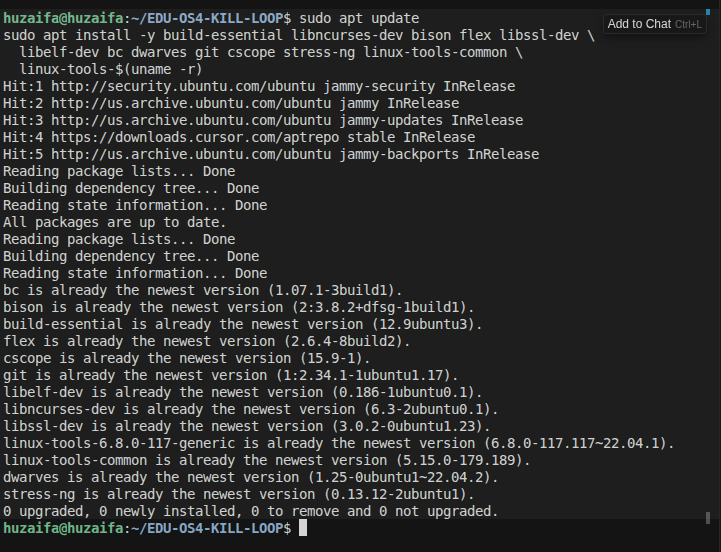
\includegraphics[width=\linewidth]{phase0-apt-deps.png}
    \caption{Installing kernel build and benchmark packages; all packages were already present on the host.}
\end{figure}

\subsection{Source Tree}

The stable kernel was cloned shallowly on branch \texttt{v6.8}, then checked out at tag \texttt{v6.8.12}:

\begin{termbox}[Clone and pin kernel tag]
\begin{lstlisting}[style=terminal]
cd /home/huzaifa/EDU-OS4-KILL-LOOP
mkdir -p kernel docs kernel/configs kernel/patches
git clone --depth=1 --branch v6.8 \
  https://git.kernel.org/pub/scm/linux/kernel/git/stable/linux.git kernel/linux
cd kernel/linux
git fetch --depth=1 origin tag v6.8.12
git checkout v6.8.12
git describe --always > ../../docs/kernel-tag.txt
\end{lstlisting}
\end{termbox}

\begin{figure}[H]
    \centering
    \includegraphics[width=\linewidth]{{phase1-clone-v6.8.12}.png}
    \caption{Cloning the stable tree and checking out tag v6.8.12 (\texttt{HEAD} at commit for Linux 6.8.12).}
\end{figure}

\subsection{Kernel Configuration}

A default x86\_64 configuration was generated and saved for reproducibility:

\begin{termbox}[defconfig]
\begin{lstlisting}[style=terminal]
cd kernel/linux
make defconfig
make olddefconfig
cp .config ../configs/config-6.8.12-baseline
\end{lstlisting}
\end{termbox}

\begin{figure}[H]
    \centering
    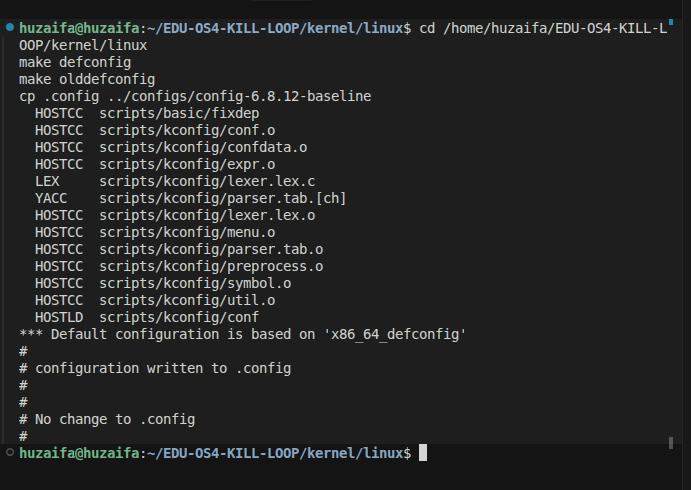
\includegraphics[width=\linewidth]{phase1-defconfig.png}
    \caption{\texttt{make defconfig} based on \texttt{x86\_64\_defconfig}; configuration written to \texttt{.config} and copied to \texttt{kernel/configs/}.}
\end{figure}

\subsection{Compilation}

The kernel was built with a distinct \texttt{LOCALVERSION} suffix so it does not collide with distribution packages:

\begin{termbox}[Build baseline kernel]
\begin{lstlisting}[style=terminal]
make -j2 LOCALVERSION=-baseline 2>&1 | tee ~/build.log
\end{lstlisting}
\end{termbox}

\begin{figure}[H]
    \centering
    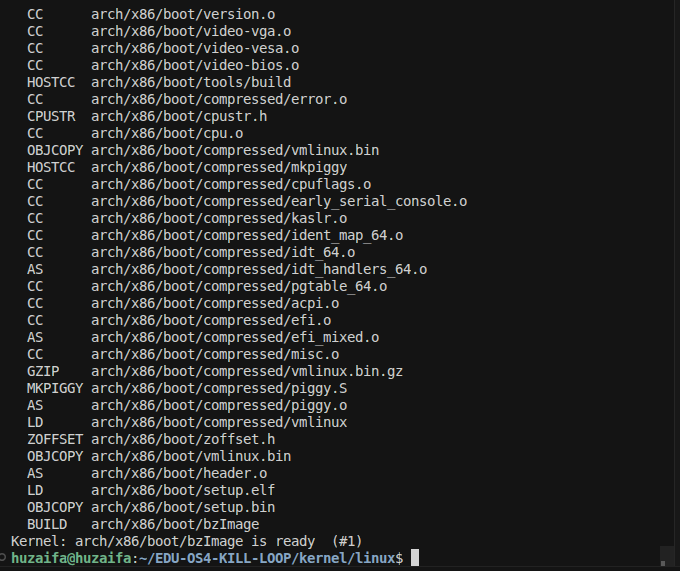
\includegraphics[width=\linewidth]{phase1-bzimage-ready.png}
    \caption{Successful build: \texttt{arch/x86/boot/bzImage} is ready for installation.}
\end{figure}

\subsection{Installation}

After a successful \texttt{make}, modules and the boot image were installed:

\begin{termbox}[Install kernel]
\begin{lstlisting}[style=terminal]
sudo make modules_install install
\end{lstlisting}
\end{termbox}

\begin{figure}[H]
    \centering
    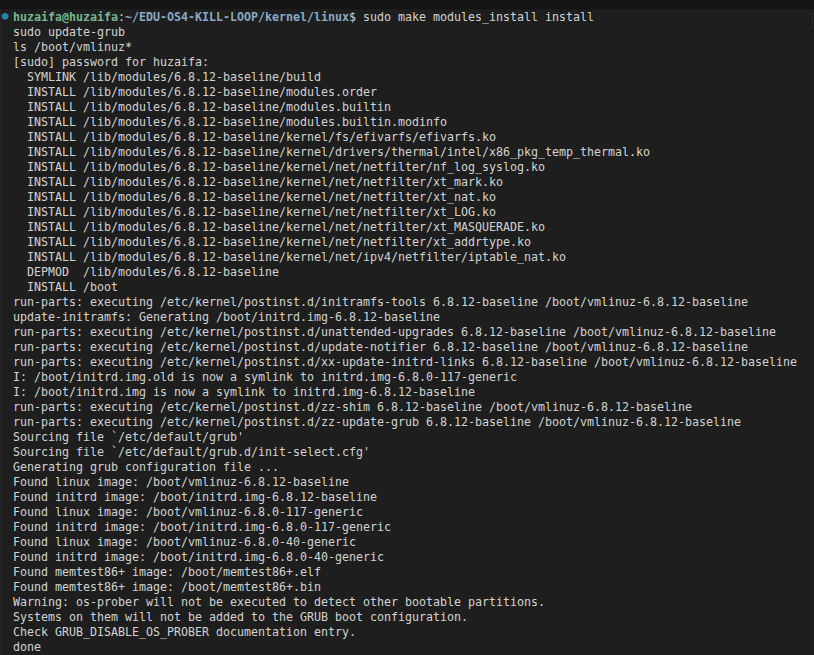
\includegraphics[width=\linewidth]{phase1-modules-install.png}
    \caption{\texttt{modules\_install} and \texttt{install} placing \texttt{vmlinuz-6.8.12-baseline} and modules under \texttt{/lib/modules/6.8.12-baseline/}.}
\end{figure}

\subsection{Bootloader Update}

GRUB was regenerated so the new kernel appears in the boot menu:

\begin{termbox}[Update GRUB]
\begin{lstlisting}[style=terminal]
sudo update-grub
ls /boot/vmlinuz*
\end{lstlisting}
\end{termbox}

\begin{figure}[H]
    \centering
    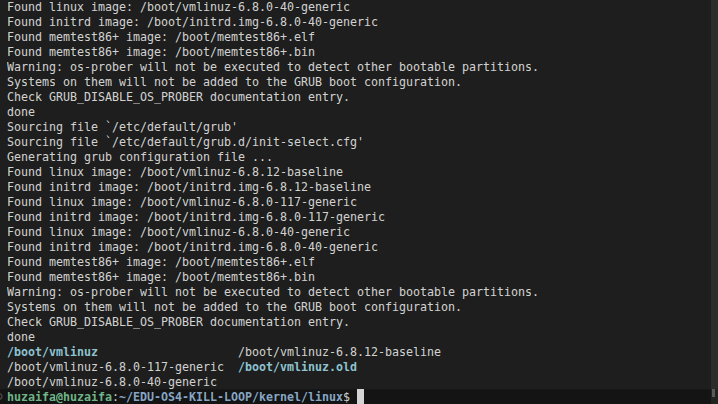
\includegraphics[width=\linewidth]{phase1-update-grub.png}
    \caption{\texttt{update-grub} detected \texttt{/boot/vmlinuz-6.8.12-baseline} alongside Ubuntu \texttt{6.8.0-117-generic} and \texttt{6.8.0-40-generic}.}
\end{figure}

\subsection{Boot Verification}

The GRUB boot menu now lists the custom baseline kernel as the first selectable entry, while the stock Ubuntu kernels remain available as fallback options.

\begin{figure}[H]
    \centering
    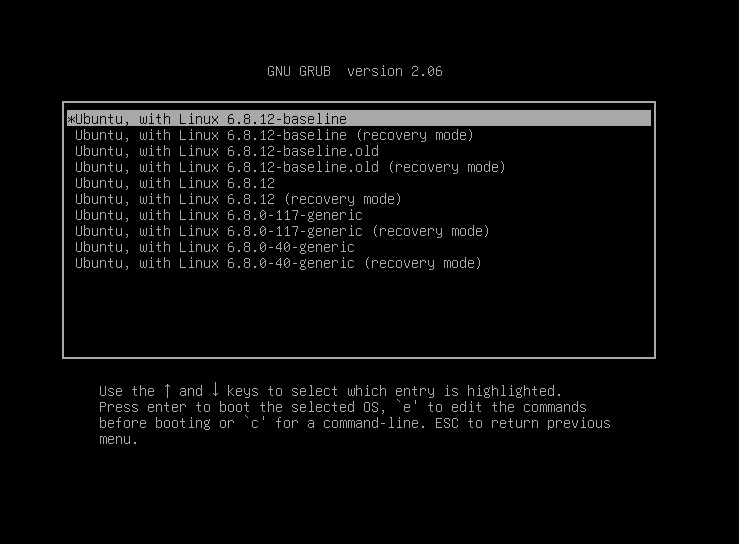
\includegraphics[width=\linewidth]{phase1-grub-menu.png}
    \caption{GRUB menu showing \texttt{Ubuntu, with Linux 6.8.12-baseline} selected, with recovery and fallback Ubuntu kernel entries still available.}
\end{figure}

Baseline install verified: \texttt{/boot/vmlinuz-6.8.12-baseline}, \texttt{/lib/modules/6.8.12-baseline/}, and GRUB entry present (see GRUB screenshot above). Select \textbf{Advanced options for Ubuntu} $\rightarrow$ \textbf{6.8.12-baseline} and confirm \texttt{uname -r} shows \texttt{6.8.12-baseline} before Phase~4 benchmarks.

\section{Component Identification}

This section satisfies the course requirement to identify the selected kernel component within the source tree. The analysis targets Linux \textbf{v6.8.12} in \texttt{kernel/linux}. A markdown companion is maintained at \texttt{docs/identification.md}.

\subsection{Selected Component}

\begin{itemize}[leftmargin=1.2cm]
    \item \textbf{Course category:} Page replacement / reclaim (PressurePause extends direct reclaim coordination).
    \item \textbf{Primary files:} \texttt{mm/page\_alloc.c} (allocation slowpath), \texttt{mm/vmscan.c} (reclaim engine).
    \item \textbf{Supporting context:} \texttt{kernel/sched/psi.c}, \texttt{include/linux/psi\_types.h} (PSI accounting).
    \item \textbf{Planned hook (Phase~3):} \texttt{do\_try\_to\_free\_pages()} in \texttt{mm/vmscan.c}, line~6188, immediately before the priority loop that calls \texttt{shrink\_zones()}.
\end{itemize}

\subsection{Call Graph: Allocation to Reclaim}

When \texttt{get\_page\_from\_freelist()} cannot satisfy an allocation (zone free pages below watermarks), control enters the allocator slowpath and eventually direct reclaim:

\begin{enumerate}[leftmargin=1.2cm]
    \item \texttt{\_\_alloc\_pages\_slowpath} --- \texttt{mm/page\_alloc.c} $\sim$4040
    \item \texttt{wake\_all\_kswapds} --- \texttt{mm/page\_alloc.c} $\sim$3814 (background reclaim hint)
    \item \texttt{\_\_alloc\_pages\_direct\_reclaim} --- \texttt{mm/page\_alloc.c} $\sim$3781
    \item \texttt{psi\_memstall\_enter} / \texttt{\_\_perform\_reclaim} --- \texttt{mm/page\_alloc.c} $\sim$3755--3790
    \item \texttt{try\_to\_free\_pages} --- \texttt{mm/vmscan.c} $\sim$6406
    \item \texttt{do\_try\_to\_free\_pages} --- \texttt{mm/vmscan.c} $\sim$6188 \textbf{[planned hook]}
    \item \texttt{shrink\_zones} $\rightarrow$ \texttt{shrink\_node} --- \texttt{mm/vmscan.c} $\sim$6065 / $\sim$5881
\end{enumerate}

\begin{center}
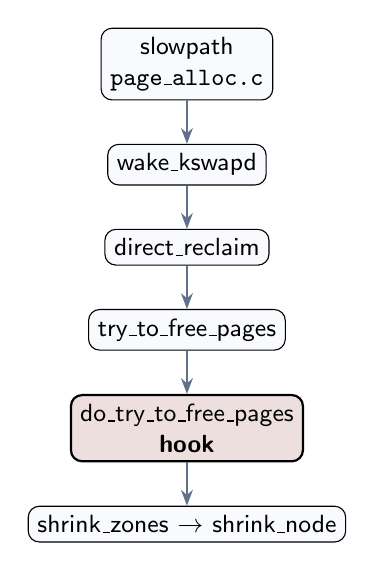
\begin{tikzpicture}[
    node distance=0.55cm and 0.3cm,
    every node/.style={font=\small\sffamily, align=center},
    arr/.style={-{Stealth[length=2mm]}, thick, color=aublue!70}
]
\node (slow) [draw, rounded corners, fill=codebg] {slowpath\\\texttt{page\_alloc.c}};
\node (wake) [draw, rounded corners, fill=codebg, below=of slow] {wake\_kswapd};
\node (direct) [draw, rounded corners, fill=codebg, below=of wake] {direct\_reclaim};
\node (try) [draw, rounded corners, fill=codebg, below=of direct] {try\_to\_free\_pages};
\node (hook) [draw, rounded corners, fill=accentgold!15, thick, below=of try] {do\_try\_to\_free\_pages\\\textbf{hook}};
\node (shrink) [draw, rounded corners, fill=codebg, below=of hook] {shrink\_zones $\rightarrow$ shrink\_node};
\draw[arr] (slow) -- (wake);
\draw[arr] (wake) -- (direct);
\draw[arr] (direct) -- (try);
\draw[arr] (try) -- (hook);
\draw[arr] (hook) -- (shrink);
\end{tikzpicture}
\end{center}

\subsection{Key Code Excerpts}

\textbf{Direct reclaim entry from the allocator} (\texttt{mm/page\_alloc.c}):

\begin{codebox}[mm/page\_alloc.c: \_\_perform\_reclaim (lines 3753--3770)]
\begin{lstlisting}[style=cstyle]
/* Perform direct synchronous page reclaim */
static unsigned long
__perform_reclaim(gfp_t gfp_mask, unsigned int order,
                  const struct alloc_context *ac)
{
    ...
    progress = try_to_free_pages(ac->zonelist, order, gfp_mask,
                                 ac->nodemask);
    ...
    return progress;
}
\end{lstlisting}
\end{codebox}

\textbf{Public direct-reclaim wrapper} (\texttt{mm/vmscan.c}):

\begin{codebox}[mm/vmscan.c: try\_to\_free\_pages (lines 6406--6446)]
\begin{lstlisting}[style=cstyle]
unsigned long try_to_free_pages(struct zonelist *zonelist, int order,
                                gfp_t gfp_mask, nodemask_t *nodemask)
{
    struct scan_control sc = { ... };
    ...
    trace_mm_vmscan_direct_reclaim_begin(order, sc.gfp_mask);
    nr_reclaimed = do_try_to_free_pages(zonelist, &sc);
    trace_mm_vmscan_direct_reclaim_end(nr_reclaimed);
    ...
    return nr_reclaimed;
}
\end{lstlisting}
\end{codebox}

\textbf{Reclaim loop and planned hook site} (\texttt{mm/vmscan.c}):

\begin{codebox}[mm/vmscan.c: do\_try\_to\_free\_pages (lines 6188--6206)]
\begin{lstlisting}[style=cstyle]
static unsigned long do_try_to_free_pages(struct zonelist *zonelist,
                                          struct scan_control *sc)
{
    ...
    do {
        sc->nr_scanned = 0;
        shrink_zones(zonelist, sc);   /* LRU eviction per zone */
        if (sc->nr_reclaimed >= sc->nr_to_reclaim)
            break;
        ...
    } while (--sc->priority >= 0);
    ...
}
\end{lstlisting}
\end{codebox}

\subsection{Watermarks}

Reclaim is triggered when a zone's free page count falls below configured \textbf{min}, \textbf{low}, or \textbf{high} watermarks during allocation. The fast path in \texttt{get\_page\_from\_freelist()} fails; \texttt{\_\_alloc\_pages\_slowpath()} may wake \texttt{kswapd}, attempt compaction, and finally call \texttt{\_\_alloc\_pages\_direct\_reclaim()} so the allocating thread performs synchronous reclaim.

\subsection{kswapd vs.\ Direct Reclaim}

Both paths converge on \texttt{shrink\_node()}, but they differ in caller context and entry points:

\begin{table}[H]
\centering
\begin{tabular}{@{}p{3.2cm}p{5.2cm}p{5.2cm}@{}}
\toprule
\textbf{Aspect} & \textbf{Direct reclaim} & \textbf{kswapd} \\
\midrule
Caller & Allocating task (slowpath) & \texttt{kswapd} kernel thread ($\sim$7078) \\
Entry & \texttt{try\_to\_free\_pages} & \texttt{balance\_pgdat} $\rightarrow$ \texttt{kswapd\_shrink\_node} \\
Shared core & \texttt{shrink\_node} & \texttt{shrink\_node} \\
GFP context & Caller's \texttt{gfp\_mask} & \texttt{GFP\_KERNEL} \\
PressurePause & Yes (hook at \texttt{do\_try\_to\_free\_pages}) & No (unless explicitly guarded) \\
\bottomrule
\end{tabular}
\caption{Comparison of foreground direct reclaim and background \texttt{kswapd}.}
\end{table}

\subsection{Pressure Stall Information (PSI)}

PSI accounts time tasks spend stalled on memory, I/O, or CPU. For PressurePause, the relevant signal is memory PSI \textbf{full}: periods when stalled tasks exist and no other tasks are making productive forward progress on memory.

\begin{itemize}[leftmargin=1.2cm]
    \item \textbf{Types:} \texttt{PSI\_MEM\_SOME}, \texttt{PSI\_MEM\_FULL} in \texttt{include/linux/psi\_types.h}
    \item \textbf{Accounting:} \texttt{kernel/sched/psi.c}
    \item \textbf{Userspace:} \texttt{/proc/pressure/memory} (\texttt{some} vs.\ \texttt{full} averages)
\end{itemize}

\texttt{psi\_memstall\_enter()} in \texttt{\_\_alloc\_pages\_direct\_reclaim} marks the \emph{current allocating task} as memory-stalled during reclaim for PSI statistics. That is distinct from reading system-wide \texttt{full} averages, which the patch will use to decide whether to apply bounded coordination before \texttt{shrink\_zones()}.

\subsection{Hook Justification}

\texttt{shrink\_node()} is shared by both \texttt{kswapd} and direct reclaim. Hooking only at \texttt{do\_try\_to\_free\_pages()} limits changes to the allocating-thread path without affecting background reclaim unless explicitly intended. Hooking at \texttt{shrink\_node()} would require \texttt{!current\_is\_kswapd()} guards and a broader behavioral surface.

Identification screenshots (editor views of \texttt{vmscan.c}, \texttt{grep} call chains, or \texttt{/proc/pressure/memory} under load) may be added in a future revision; this section relies on verified line numbers from the v6.8.12 tree.

\section{Design and Alternative Methodologies}

\textbf{Chosen approach:} PSI-gated bounded backoff on direct reclaim entry---wake \texttt{kswapd}, wait up to \texttt{PRESSURE\_PAUSE\_MAX\_MS}, then fall through to stock reclaim on timeout or lack of progress.

\begin{table}[H]
\centering
\begin{tabular}{@{}p{3.5cm}p{5cm}p{5cm}@{}}
\toprule
\textbf{Approach} & \textbf{Pros} & \textbf{Cons} \\
\midrule
A. PSI-gated backoff (chosen) & Uses kernel stall signal; small code surface & Lock-context constraints; must validate no regressions \\
B. Fixed sleep in reclaim & Simple to implement & Blind to real pressure; may delay recovery \\
C. User-space only (swappiness, cgroups) & No kernel patch risk & Does not satisfy course kernel-modification requirement \\
\bottomrule
\end{tabular}
\caption{Alternative methodologies considered for coordinating reclaim under thrash.}
\end{table}

Constants in \texttt{mm/vmscan.c}: \texttt{PSI\_MEM\_THRESHOLD\_BPS=1} (0.01\% stall, fixed-point compare via \texttt{psi\_mem\_avg10\_exceeds\_bps()}), \texttt{PRESSURE\_PAUSE\_MAX\_MS=20}. Activation and skip counters: \texttt{/sys/kernel/debug/pressure\_pause\_activations}.

\section{Implementation}

The patch is exported as \texttt{kernel/patches/0001-pressurepause.patch} on branch \texttt{pressurepause} in \texttt{kernel/linux}. Config with \texttt{CONFIG\_PSI=y} and \texttt{CONFIG\_LOCALVERSION="-pressurepause"} is saved as \texttt{kernel/configs/config-6.8.12-pressurepause}.

\subsection{Files changed}

\begin{itemize}[leftmargin=1.2cm]
    \item \texttt{include/linux/psi.h} --- \texttt{psi\_mem\_full\_avg10()}, \texttt{psi\_mem\_some\_avg10()}
    \item \texttt{kernel/sched/psi.c} --- read system memory PSI \texttt{some}/\texttt{full} avg10 (same locking path as \texttt{psi\_show()})
    \item \texttt{mm/vmscan.c} --- \texttt{pressure\_pause\_maybe()} at \texttt{do\_try\_to\_free\_pages()} entry (before \texttt{shrink\_zones} loop)
\end{itemize}

\subsection{PSI threshold fix}

The initial gate used \texttt{LOAD\_INT(psi\_full) >= 25}, which requires \textbf{25\%} memory \texttt{full} stall (the integer part of the fixed-point average matches the whole-number in \texttt{/proc/pressure/memory}, e.g.\ \texttt{avg10=25.00}). Benchmarks peaked near \texttt{full avg10=0.18} (0.18\%), so the patch never ran. The fix uses \texttt{psi\_mem\_avg10\_exceeds\_bps()} with \texttt{PSI\_MEM\_THRESHOLD\_BPS=1} (0.01\%) on memory PSI \texttt{some} avg10, which rises earlier than \texttt{full} under swap-heavy thrash. Debugfs reports \texttt{activations}, per-guard \texttt{skip\_*} counts, and \texttt{peak\_psi\_*} maxima seen at the hook.

\subsection{Control flow}

When direct reclaim enters \texttt{do\_try\_to\_free\_pages()}:
\begin{enumerate}[leftmargin=1.2cm]
    \item If cgroup reclaim, or PSI \texttt{some} avg10 below 0.01\%, or no reclaimable pages, or no zone below min watermarks $\rightarrow$ stock path.
    \item Else wake \texttt{kswapd} for each zone in the zonelist via \texttt{wakeup\_kswapd()}.
    \item Bounded wait (max 20\,ms): exit early if watermarks improve or on fatal signal; always continue to \texttt{shrink\_zones()}.
\end{enumerate}

\subsection{Build and install}

\begin{codebox}[Build patched kernel]
\begin{lstlisting}[style=bashstyle]
cd kernel/linux
git checkout pressurepause
scripts/config --enable PSI
scripts/config --set-str LOCALVERSION "-pressurepause"
make olddefconfig && make -j2
./scripts/install-pressurepause-kernel.sh   # or: sudo make modules_install install && sudo update-grub
\end{lstlisting}
\end{codebox}

\textbf{Boot verification:} GRUB $\rightarrow$ Advanced options $\rightarrow$ \texttt{6.8.12-pressurepause} (or \texttt{6.8.12-pressurepause+} if built from a dirty tree). Confirm \texttt{uname -r}, \texttt{cat /proc/pressure/memory}, and \texttt{./scripts/verify-activation.sh}. The patched kernel was booted successfully, memory PSI was available, repeated 120\,s \texttt{stress-ng} virtual-memory workloads completed without crash or hang, and the debugfs counter confirmed real PressurePause executions during benchmark runs.

\subsection{Evaluation (benchmarks)}

Comparative runs use \texttt{./bench-run.sh} on \texttt{6.8.12-baseline} (before) and \texttt{6.8.12-pressurepause+} (after), saving timestamped directories under \texttt{results/}. Metrics: \texttt{pgmajfault} delta, \texttt{vmstat} \texttt{si}/\texttt{so}, PSI samples during stress, and on the patched kernel \texttt{pressure-pause-debugfs-*.txt}. Final patched runs show \texttt{activations} increases of +40 on the 8-worker/93\% workload and +15 on one 4-worker/85\% workload, proving that the reclaim coordination path executed.

\section{Correctness and Safety}

\begin{enumerate}[leftmargin=1.2cm]
    \item \textbf{Bounded wait:} \texttt{PRESSURE\_PAUSE\_MAX\_MS} caps the coordination loop; uses \texttt{schedule\_timeout\_idle(1)} slices.
    \item \textbf{Never skip reclaim:} \texttt{pressure\_pause\_maybe()} always returns; stock \texttt{shrink\_zones()} priority loop runs afterward.
    \item \textbf{kswapd cooperation:} \texttt{wakeup\_kswapd()} is additive; foreground reclaim still proceeds.
    \item \textbf{Livelock guard:} skip pause if \texttt{zone\_reclaimable\_pages()} is zero for all zones in the zonelist.
    \item \textbf{Fallback:} Ubuntu \texttt{6.8.0-117-generic} and \texttt{6.8.12-baseline} remain in GRUB if the patched kernel panics.
\end{enumerate}

\section{Evaluation}

\subsection{Methodology}

Matched pairs on the same host used \texttt{./bench-run.sh} with \texttt{stress-ng --vm N --vm-bytes P\% --timeout 120s}, \texttt{vmstat}, \texttt{pgmajfault}, PSI samples, and debugfs PressurePause counters. Representative directories: 8 workers / 93\% --- baseline \texttt{bench-6.8.12-baseline-20260519-135148} vs patched \texttt{bench-6.8.12-pressurepause+-20260519-155900}; 4 workers / 85\% --- baseline \texttt{bench-6.8.12-baseline-20260519-135638} vs patched average of \texttt{160116}, \texttt{160400}, and \texttt{160617}.

\begin{table}[H]
\centering
\begin{tabular}{@{}lccc@{}}
\toprule
\textbf{Workload} & \textbf{Metric} & \textbf{Baseline} & \textbf{PressurePause+} \\
\midrule
8 vm / 93\% & Avg swap-out (KB/s) & 31222.5 & 25638.6 \\
8 vm / 93\% & End swap (KB) & 37992 & 25952 \\
8 vm / 93\% & \texttt{activations} $\Delta$ & -- & +40 \\
8 vm / 93\% & \texttt{pgmajfault} $\Delta$ & 222 & 321 \\
4 vm / 85\% & Avg swap-out (KB/s) & 33380.0 & 22791.8 \\
4 vm / 85\% & Max swapped (KB) & 1215952 & 913977.3 \\
4 vm / 85\% & End swap (KB) & 91676 & 26104 \\
4 vm / 85\% & \texttt{activations} $\Delta$ & -- & +15 total \\
4 vm / 85\% & \texttt{pgmajfault} $\Delta$ & 5 & 112.7 \\
\bottomrule
\end{tabular}
\caption{Matched benchmark summary (May 2026). Patched runs used the rebuilt PressurePause+ kernel with debugfs activation counters. The 4 vm / 85\% patched column averages three patched trials.}
\end{table}

\subsection{Discussion}

After correcting the PSI gate (25\% \texttt{LOAD\_INT} bug $\rightarrow$ 0.01\% \texttt{some} avg10), PressurePause now both activates and improves the main swap-pressure metrics. On the 8\,vm / 93\% workload, the debugfs counter increased from 15 to 55 (+40 activations), average swap-out fell by 17.9\%, and residual swap fell by 31.7\%. On the 4\,vm / 85\% workload, the three-run patched average reduced average swap-out by 31.7\%, maximum swapped memory by 24.8\%, and residual swap by 71.5\%; run \texttt{160617} also confirmed +15 PressurePause activations. The tradeoff remains higher \texttt{pgmajfault} on patched runs, so the strongest claim is improved swap pressure with a documented page-fault cost.

\subsection{Limitations}

This is not a full statistical study. PSI samples are every 5\,s and can miss short spikes seen at the reclaim hook, which is why the debugfs activation counter is more important than sampled \texttt{avg10} alone. Baseline PSI still reports ``no PSI,'' so baseline and patched PSI totals cannot be compared directly. Major-fault counts rise on the patched kernel; future work should add repeated trials, latency percentiles, and a workload sweep to find where the swap reduction is worth the fault-cost tradeoff.

\section{Conclusion}

The baseline Linux~v6.8.12 kernel and the PressurePause patch (\texttt{6.8.12-pressurepause+}) were built and compared under controlled \texttt{stress-ng} workloads. The final runs confirm that the patched reclaim path executes: PressurePause activated +40 times in the 8\,vm / 93\% workload and +15 times in one 4\,vm / 85\% workload. The modification is stable and reduces swap pressure in matched benchmarks, with average swap-out falling by 17.9\% on 8\,vm / 93\% and by 31.7\% on the 4\,vm / 85\% average. The remaining tradeoff is increased major page faults, so the project demonstrates PSI-gated, bounded direct-reclaim coordination with measurable swap benefits and a documented fault-count cost.

\end{document}
